%%%%%%%%%%%%%%%%%%%%%%%%%%%%%%%%%%%%%%%%%
% Software Engineering Process
% LaTeX Template
% Version 1.0 (12/08/2019)
%%%%%%%%%%%%%%%%%%%%%%%%%%%%%%%%%%%%%%%%%


\documentclass[final]{beamer}

\usepackage[scale=1.24]{beamerposter} % Use the beamerposter package for laying out the poster

%\usetheme{confposter} % Use the confposter theme supplied with this template
\usetheme[faculty=phil]{fibeamer} % Uncomment to use Masaryk University's fibeamer theme instead.



\newlength{\sepwid}
\newlength{\onecolwid}
\newlength{\twocolwid}
\newlength{\threecolwid}
\setlength{\paperwidth}{46.8in} % A0 width: 46.8in
\setlength{\paperheight}{33.1in} % A0 height: 33.1in
\setlength{\sepwid}{0.024\paperwidth} % Separation width (white space) between columns
\setlength{\onecolwid}{0.21\paperwidth} % Width of one column
\setlength{\twocolwid}{0.451\paperwidth} % Width of two columns
\setlength{\threecolwid}{0.678\paperwidth} % Width of three columns
%\setlength{\topmargin}{-0.5in} % Reduce the top margin size
%-----------------------------------------------------------

\usepackage{graphicx}  % Required for including images

\usepackage{booktabs} % Top and bottom rules for tables

%----------------------------------------------------------------------------------------
%	TITLE SECTION 
%----------------------------------------------------------------------------------------

\title{Poster Presentation: Gamma Function: Team I} % Poster title

\author{Amit Sachdeva, 40084627} % Author(s)

\institute{ Master of Software Engineering, Concordia University} % Institution(s)

%----------------------------------------------------------------------------------------

\begin{document}
\addtobeamertemplate{block end}{}{\vspace*{2ex}} % White space under blocks
\addtobeamertemplate{block example end}{}{\vspace*{2ex}} % White space under example blocks
\addtobeamertemplate{block alerted end}{}{\vspace*{2ex}} % White space under highlighted (alert) blocks

\setlength{\belowcaptionskip}{2ex} % White space under figures
\setlength\belowdisplayshortskip{2ex} % White space under equations
%\begin{darkframes} % Uncomment for dark theme, don't forget to \end{darkframes}
\begin{frame} % The whole poster is enclosed in one beamer frame

%==========================Begin Head===============================

  \begin{columns}
   \begin{column}{\linewidth}
    \vskip1cm
    \centering
    \usebeamercolor{title in headline}{\color{fg}\Huge{\textbf{\inserttitle}}\\[0.5ex]}
    \usebeamercolor{author in headline}{\color{fg}\Large{\insertauthor}\\[1ex]}
    \usebeamercolor{institute in headline}{\color{fg}\large{\insertinstitute}\\[1ex]}
    \vskip1cm
   \end{column}
   \vspace{1cm}
  \end{columns}
 \vspace{1cm}

%==========================End Head===============================

\begin{columns}[t] % The whole poster consists of three major columns, the second of which is split into two columns twice - the [t] option aligns each column's content to the top

\begin{column}{\sepwid}\end{column} % Empty spacer column

\begin{column}{\onecolwid} % The first column

%----------------------------------------------------------------------------------------
%	OBJECTIVES
%----------------------------------------------------------------------------------------

\begin{exampleblock}{Objectives}

\small{This project is about the functionality of gamma function as well as proper documentation. User can insert any real value and expect real value except on boundary conditions. Firstly, requirements and assumptions are made for our function and best algorithm is decided out of two different algorithms. Target is not limited to functionality but to improve user experience but keeping in mind about the proper coding style. Code reviewing is also done to get know the weak points. }

\end{exampleblock}

%----------------------------------------------------------------------------------------
%	INTRODUCTION
%----------------------------------------------------------------------------------------

\begin{exampleblock}{Introduction}
\small{\textbf{Gamma Function: } It is commonly referred as factorial function for complex numbers. It is derived by Daniel Bernoulli. The gamma function $\Gamma(z)$ is defined for all complex values of z larger than zero. Complex number can be consist of real and imaginary number, like $z = a + i b$ in which a and b can real numbers. A complex number is typically written in the form where sigma a is the real part and it is the imaginary part. \textbf{Range} of the function is $(0,\inf)$ and \textbf{Domain} is from $[0, 109]$}
\end{exampleblock}

%------------------------------------------------

\begin{figure}
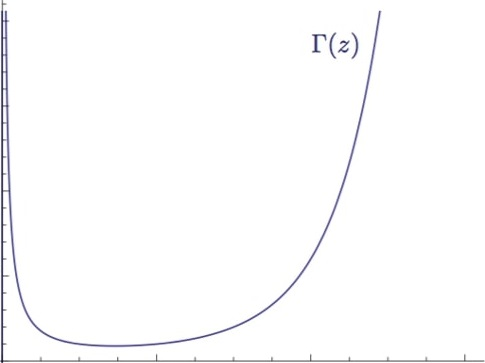
\includegraphics[width=0.5\linewidth]{img/d4_2.jpg}
\caption{Gamma Function}
\label{fig:Gamma Function}
\end{figure}

\begin{figure}
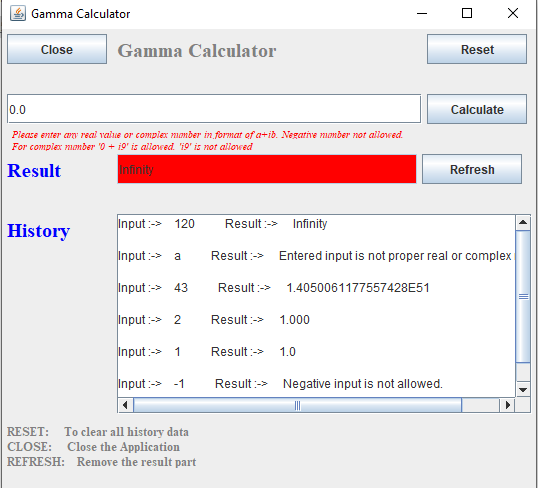
\includegraphics[width=0.8\linewidth]{img/d4_1.png}
\caption{GUI of Gamma Function}
\label{fig:GUI of Gamma Function}
\end{figure}

%----------------------------------------------------------------------------------------

\end{column} % End of the first column

\begin{column}{\sepwid}\end{column} % Empty spacer column

\begin{column}{\twocolwid} % Begin a column which is two columns wide (column 2)

\begin{columns}[t,totalwidth=\twocolwid] % Split up the two columns wide column

\begin{column}{\onecolwid}\vspace{-.74in} % The first column within column 2 (column 2.1)

%----------------------------------------------------------------------------------------
%	MATERIALS
%----------------------------------------------------------------------------------------

\begin{exampleblock}{Pseudo code}
\small{This algorithm is based on calculating based on using core integral using graph like dividing whole graph in small parts and calculating each part using formula of trapezium \textbf{($ 1/2*(base1 + base2)*height $)} and combining it at the end. We can get more precise results using this algorithm.  \newline\newline
function yAxisValue(Argument x, Argument s) \{ \newline 
\hspace*{20pt}calculate the value using $value = {s^{x - 1} e^{ - s}}$\newline
\hspace*{20pt}return value\newline
end \newline
\}  \newline
function gammaFunction (Argument x) \{ \newline
\hspace*{20pt} if x $<$ 0\newline
\hspace*{50pt} then raise Negative Input Error\newline
\hspace*{20pt} if x $>$ 110\newline
\hspace*{50pt} then return "Infinity"\newline
\hspace*{20pt} Initialize finalData with 0\newline
\hspace*{20pt} Set Interval for gap = $10 ^ {-3}$ \newline
\hspace*{20pt} while loop i for range (0,Infinity)\newline
\hspace*{50pt} add the finalData by using formula of trapezium using \newline 
\hspace*{50pt} \textbf{$1/2*gap*(yAxisValue(i) + yAxisValue(i-gap))$} \newline
\hspace*{50pt} increment i with gap value \newline
\hspace*{20pt} return finalData\newline
end \newline
\} \{ \newline
In main function \newline
\hspace*{20pt} Take a input of x \newline
\hspace*{20pt} Call gammaFunction with input x-1 as a argument \newline
end
\}}
\end{exampleblock}
\begin{exampleblock}{Requirements and Assumptions}
\begin{itemize}
    \small{\item  For \textbf{Large input} in positive real value, it will return infinity $\forall$ values $>$ 110.
    \item  For \textbf{negative input} $\forall x<0 $, \textbf{Function} will return \textbf{negative input error}.
    \item  For \textbf{$x=0$}, \textbf{Function} will return \textbf{1}
    \item  For \textbf{$Re(x) > 0$}, \textbf{Function} will return positive real value, keeping in mind values belongs to real value}
    \item For invalid string like: any string, or wrong complex number like i9, \textbf{Function} will return \textbf{Wrong input error}
\end{itemize}

\end{exampleblock}
%----------------------------------------------------------------------------------------

\end{column} % End of column 2.1

\begin{column}{\onecolwid}\vspace{-.74in} % The second column within column 2 (column 2.2)


\begin{exampleblock}{Coding Conventions and Additional things}

\small{\textbf{\underline{Coding Convention}}
\begin{enumerate}
    \item Methods and variables should be in Camel Case. 
    \item Class name should be start with capital letter.
    \item Package should be in capital letter.
    \item Function length should be less than 30 words.
    \item Constant should be of capital letters.
\end{enumerate}

\textbf{\underline{Additional Things}}
\begin{enumerate}
    \item \textbf{JUnit 4} For Testing the functionality of project. 
    \item \textbf{Eclipse} is used as debugger.
    \item \textbf{Check style} is used to improve code quality.
    \item \textbf{Java Docs} for documentation and working of methods
\end{enumerate}}




\end{exampleblock}
\begin{figure}
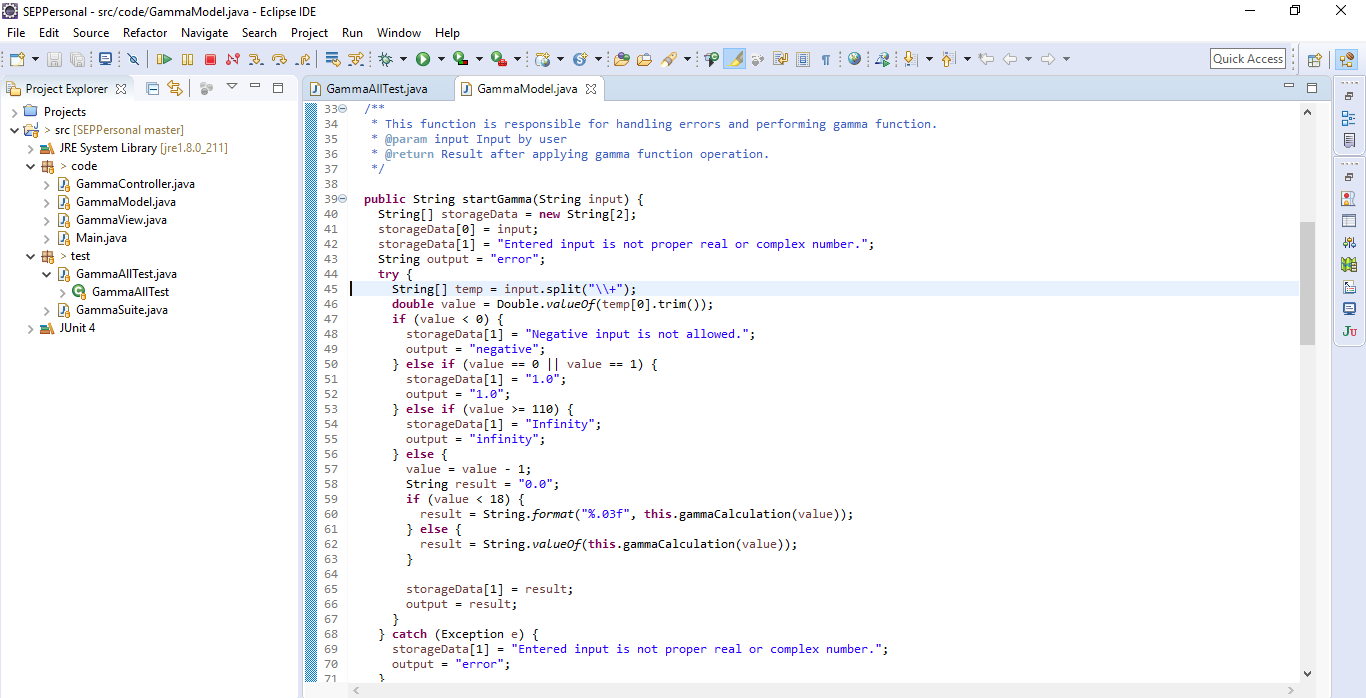
\includegraphics[width=0.6\linewidth]{img/d4_3.png}
\caption{All Test Cases}
\label{fig:All Test Cases}
\end{figure}

\begin{figure}
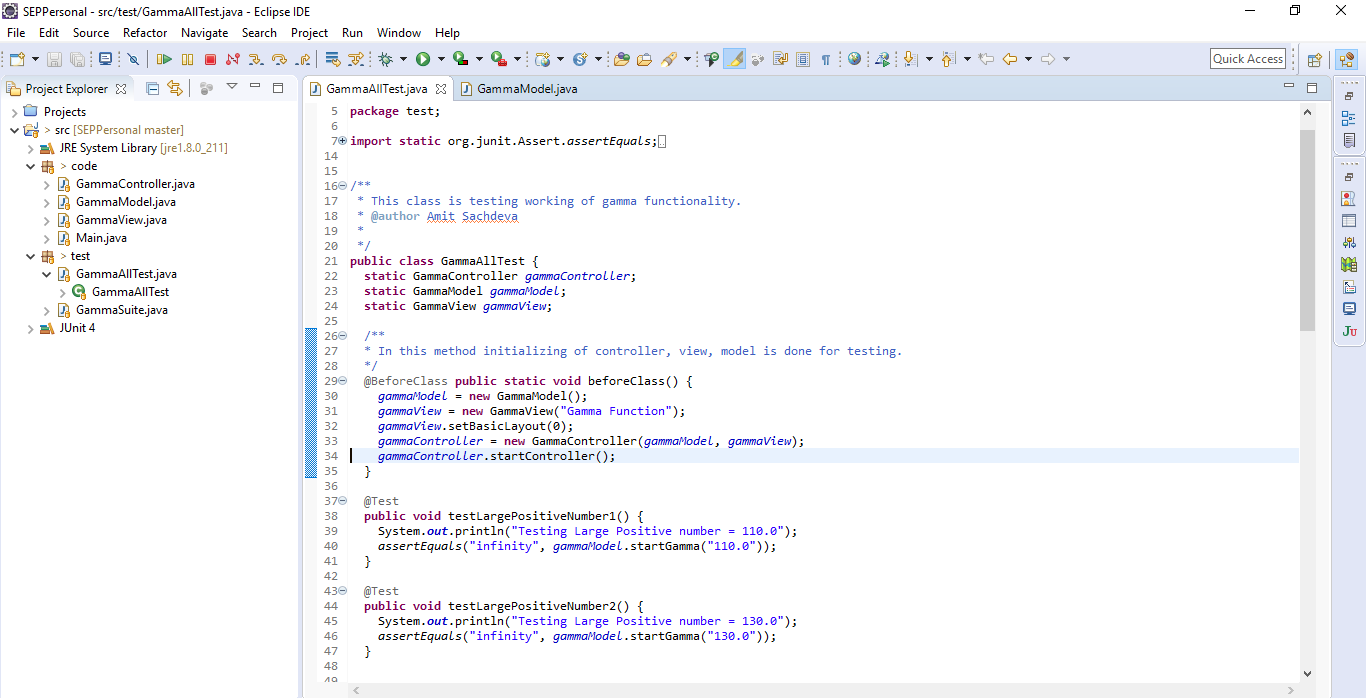
\includegraphics[width=0.6\linewidth]{img/d4_4.png}
\caption{Coding style and Java docs}
\label{fig:Coding style and Java docs}
\end{figure}

\begin{exampleblock}{Results}
\begin{tabular}{|p{5cm}|p{11cm}|p{8cm}|}

 \hline
 Input & Code output &Real Output\\
 \hline
 6  & 120.000  &  120\\
 99  &  8.13936\textbf{E153}  &  9.4268904\textbf{E153}\\
 0  & 1.0  &  1\\
 3+i9  & 2.000  &  2\\
 i9  & Wrong Input Error & Error \\
 -1 & Negative Input Error & Error \\
 abc & Wrong Input Error & Error\\
 120 & Infinity & Infinity \\
 \hline
\end{tabular}
\end{exampleblock}
%----------------------------------------------------------------------------------------

\end{column} % End of column 2.2

\end{columns} % End of the split of column 2 - any content after this will now take up 2 columns width



\begin{columns}[t,totalwidth=\twocolwid] % Split up the two columns wide column again


\begin{column}{\sepwid}\end{column} % Empty spacer column

\begin{column}{\onecolwid} % The second column within column 2 (column 2.2)


\end{column} % End of column 2.2

\end{columns} % End of the split of column 2

\end{column} % End of the second column

\begin{column}{\sepwid}\end{column} % Empty spacer column

\begin{column}{\onecolwid} % The third column

%----------------------------------------------------------------------------------------
%	CONCLUSION
%----------------------------------------------------------------------------------------

\begin{exampleblock}{Explicit Efforts}
\small{For this project, GUI is used to increase usability with proper exception handling to increase robustness. To enhance maintainability, Design pattern is used. Even each method has different functionality to decrease dependability. Core method of integration is implemented for gamma function which enhances efficiency and correctness.}


\end{exampleblock}


\begin{exampleblock}{Suggested Improvements and Conclusion}
\small{
\textbf{\underline{Suggested Improvements}}
\begin{itemize}
\item Java docs can be used for test cases to enhance better readability of test cases.
\item Functions length in few cases can be reduced to 20 to 30 lines to enhance the maintainability.
\item More arithmetic functions like addition, subtraction can be added to cover all aspects of calculator.
\end{itemize}
Concluding that, this project has increased the way of handling project along with proper documentation and proper coding style. It also helps in working in a team. Not only that, it also helps to maintain track of working using git, and requirement gathering at initial stage is mandatory.}
\end{exampleblock}



\begin{exampleblock}{References}

\small{\begin{itemize}
\item  https://www.ncbi.nlm.nih.gov/pmc/articles/PMC 4247832/
\item https://medium.com/cantors-paradise/the-riemann-hypothesis-explained-fa01c1f75d3f
\item https://www.quora.com/What-are-the-advantages-of-Eclipse-IDE
\item https://checkstyle.org/eclipse-cs/
\item https://www.eclipse.org/forums/index.php/t/206312/
\end{itemize}}
\end{exampleblock}



\begin{block}{Contact Information}

\small{\begin{itemize}
\item Name: Amit Sachdeva
\item Student Id: 40084627
\item Github: \url{https://github.com/amitsachdeva45/SEPPersonal/tree/master/Documentation/Deliverable4}
\item Professor: P. Kamthan
\end{itemize}}

\end{block}


%----------------------------------------------------------------------------------------

\end{column} % End of the third column

\begin{column}{\sepwid}\end{column} % Empty spacer column

\end{columns} % End of all the columns in the poster

\end{frame} % End of the enclosing frame
%\end{darkframes} % Uncomment for dark theme
\end{document}
